\documentclass{beamer}

\usetheme{Singapore}
\usecolortheme{rose}
\setbeamertemplate{blocks}[rounded][shadow=true]

\usepackage[utf8]{inputenc}
\usepackage[vietnamese]{babel}

\setbeamertemplate{footline}[frame number]

% Adding todo notes
\usepackage{todonotes}
\presetkeys{todonotes}{inline}{}

% Add color text
\usepackage{xcolor}
\definecolor{olive}{rgb}{0.3, 0.4, .1}
\definecolor{fore}{RGB}{249,242,215}
\definecolor{back}{RGB}{51,51,51}
\definecolor{title}{RGB}{255,0,90}
\definecolor{dgreen}{rgb}{0.,0.6,0.}
\definecolor{gold}{rgb}{1.,0.84,0.}
\definecolor{JungleGreen}{cmyk}{0.99,0,0.52,0}
\definecolor{BlueGreen}{cmyk}{0.85,0,0.33,0}
\definecolor{RawSienna}{cmyk}{0,0.72,1,0.45}
\definecolor{Magenta}{cmyk}{0,1,0,0}

% Cấu hình table và nhập code
\usepackage{tabu,color,listings}
\definecolor{dkgreen}{rgb}{0,0.6,0}
\definecolor{gray}{rgb}{0.5,0.5,0.5}
\definecolor{mauve}{rgb}{0.58,0,0.82}
\lstset{inputpath=Filecodes}
\lstset{frame=none,
	language=[Sharp]C,
	aboveskip=3mm,
	belowskip=3mm,
	showstringspaces=false,
	columns=flexible,
	basicstyle={\small\ttfamily},
	numbers=none,
	numberstyle=\tiny\color{gray},
	keywordstyle=\color{blue},
	commentstyle=\color{dkgreen},
	stringstyle=\color{mauve},
	breaklines=true,
	breakatwhitespace=true,
	tabsize=3
}

% Sử dụng gói algorithm2e để viết thuật toán
\usepackage{algorithm2e}

% Tham chiếu tài liệu tham khảo
\usepackage[round]{natbib} 
\bibliographystyle{plainnat}

\title{ĐỘ TƯƠNG TỰ HÀNH VI CỦA CHƯƠNG TRÌNH VÀ THỰC NGHIỆM}
\author{Đỗ Đăng Khoa}
\institute{KHMT K19 -- ĐHQN}
\date{Quy Nhơn, 25--08--2017}

\begin{document}

\begin{frame}
  \titlepage
\end{frame}

\part{}

\begin{frame}
  \frametitle{Nội dung}
  \tableofcontents{}
\end{frame}

\section{Giới thiệu}

\begin{frame}
  \frametitle{Học trực tuyến}
  \begin{minipage}{0.39\linewidth}
    
\includegraphics[width=0.9\linewidth]{images/topMOOC.png}
  \end{minipage}\hfill
  \pause
  \begin{minipage}{0.59\linewidth}
    \begin{itemize}
    \item Một số vấn đề
      \begin{itemize}
      \item Người dạy ít, người học đông
      \item Tốn thời gian đọc mã lệnh
      \item Đánh giá, xếp hạng
      \end{itemize} \pause
    \item $\rightarrow$ Cần công cụ hỗ trợ tự động
    \end{itemize} \pause
  \end{minipage}
  \begin{block}{Vấn đề cốt lõi}
    Đo được độ tương tự về hành vi giữa hai chương trình
  \end{block}
\end{frame}

\begin{frame}
  \frametitle{Một số nghiên cứu liên quan}
%  \todo{Viết gọn, chi tiết khi trình bày}
  \begin{itemize}
  \item Xếp hạng tự động: \cite{alur2013automated}
    \begin{itemize}
    \item Sử dụng khái niệm về độ tương tự về
      ngữ nghĩa dùng cho DFA; 
	\item Các độ đo dùng cho các chương trình máy tính
    \end{itemize}
  \item Kiểm tra sự tương đương: \cite{jiang2009automatic}
    \begin{itemize}
%    \item \cite{bates1993incremental} sử dụng đồ thị phụ thuộc; 
%    \item Luận văn tính độ tương tự 
    \item Sử dụng các phép thử ngẫu nhiên
    \item Tương tự phép đo RS, khác phép đo SSE và PSE
    \end{itemize}
  \item Phát hiện đạo code: \cite{komondoor2001using}
    \begin{itemize}
    \item Phân tích tĩnh các đoạn mã lệnh
	\item Thực thi chương trình, sinh dữ liệu vào/ra
    \end{itemize}
  \end{itemize}

\end{frame}

\begin{frame}
  \frametitle{Dynamic Symbolic Execution}
%  \todo{Đọc lại thật kỹ DSE, diễn đạt lại cho tốt hơn, giải thích ví dụ chưa ổn, hãy cẩn trọng, thêm ý tạo dữ liệu thử bằng cách duyệt tất cả các nhánh của chương trình}

	\begin{block}{}
		\begin{itemize}
			\item Duyệt tự động tất cả các nhánh đường đi của chương trình
			\item Thực thi chương trình với các giá trị biểu trưng
			\item Ghi nhận ràng buộc tại các nút rẽ nhánh
			\item Giải các ràng buộc tìm giá trị đầu vào
		\end{itemize}
	\end{block}
 \pause
	
  \begin{block}{Cách thức hoạt động}
    \begin{minipage}[T]{0.40\linewidth}
      \lstinputlisting[basicstyle=\footnotesize]{test_me.cs}
    \end{minipage}
    \hfill    
    \begin{minipage}[T]{0.55\linewidth}
		{\footnotesize\centering
		\begin{tabular}{  m{4em} | m{4em} | m{4em}  }
		concrete state & symbolic state & path condition \\ 
		\hline
		$ x = 0 $ & $ x = x_{0} $ & $ x_{0} != 10 $ \\  
		\hline
		$ x = 10 $ & $ x = x_{0} $ & $ x_{0} == 10 $ \\ 		
		\end{tabular}
		\\ \pause
		Kết quả sau hai lần thực thi: $ 0, 10 $ 
		}
    \end{minipage}
  \end{block}
	
\end{frame}

\section{Tương tự về hành vi của chương trình}

\begin{frame}
  \frametitle{Hai chương trình tương đương}
% \todo{Viền code cho đẹp hơn, giản lược code}
  \begin{minipage}[t]{0.40\linewidth}
    \lstinputlisting[basicstyle=\footnotesize]{SwitchCase.cs}
  \end{minipage}
  \hfill\vrule\hfill
  \begin{minipage}[t]{0.40\linewidth}
    \lstinputlisting[basicstyle=\footnotesize]{IfElse.cs}
  \end{minipage}
\pause
  \begin{block}{}
  	\centering
	Hai chương trình khác cú pháp, tương đương về hành vi
  \end{block}
\end{frame}


\begin{frame}
  \frametitle{Thực thi của một chương trình}
%  \todo{Tìm cách trình bày lại tất cả các định nghĩa cho đẹp hơn, dễ đọc hơn}
\begin{block}{}
	\begin{itemize}
		\item Cho $P$ là chương trình có tập các giá trị đầu vào $I$
		\item $O$ là tập hợp các giá trị đầu ra của $P$. 
		\item Thực thi chương trình $ P $ là ánh xạ: 
		\[exec: P \times I \rightarrow O\]
		\item Với $i \in I$, $exec(P, i) = o$, trong đó $o \in O$
	\end{itemize}
\end{block}
   
\end{frame}


\begin{frame}
  \frametitle{Tương đương về hành vi của 2 chương trình}
  \begin{block}{}
  	\begin{itemize}
  		\item Cho $P_r$ và $P_s$ là hai chương trình có cùng miền vào $I$ 
  		\item Hai chương trình này được gọi là tương đương khi và chỉ
  		khi thực thi của chúng giống nhau trên mọi giá trị đầu vào trên $I$
  		\[exec(P_r, I) = exec(P_s, I).\]
  	\end{itemize}
  \end{block} 
\end{frame}


\begin{frame}
  \frametitle{Sự khác biệt hành vi}
  \begin{block}{}
  \begin{itemize}
  	\item Cho $P_r$ và $P_s$ là hai chương trình có cùng miền vào $I$ 
  	\item Hai chương trình này được xem là có sự khác biệt về
  	hành vi khi và chỉ khi thực thi của chúng khác nhau trên một vài giá
  	trị đầu vào $i \in I$
  	\[exec(P_r, I) \neq exec(P_s, I)\]
  \end{itemize}
  \end{block}
\end{frame}


\begin{frame}
  \frametitle{Độ tương tự về hành vi}
%  \todo{Không được để rớt 1 2 chữ trên 1 dòng}
  \begin{block}{}
  	\begin{itemize}
  		\item Cho $P_r$ và $P_s$ là hai chương trình có cùng miền
  		vào $I$
  		\item Gọi $I_{s} \subseteq I$ sao cho 
  		\[\begin{cases}
  			exec(P_r, I_{s}) = exec(P_s, I_{s})\\
  			\forall j \in I \setminus I_{s}, exec(P_r, j) \neq exec(P_s, j)			
  		\end{cases}
  		\]
  		\item Độ tương tự về hành vi giữa $P_r$ và $P_s$ là: $|I_s|/|I|$.
  	\end{itemize}
  \end{block}
  
\end{frame}


\section{Đo độ tương tự về hành vi}
\begin{frame}
  \frametitle{Lấy mẫu ngẫu nhiên}
  \begin{itemize}  	
  	\item Lấy ngẫu nhiên một số giá trị trên miền vào \\(\emph{Random
  		Sampling -- RS})
  	\item Tính số lượng giá trị hai chương trình
  	thực thi giống nhau
%  	\todo{Không viết nhiều chữ, viết công thức toán học cho hình thức hóa}
  \end{itemize}
  	\begin{block}{Mô tả hình thức}
	\begin{itemize}
		\item $P_r$ và $P_s$ cùng miền vào $I$
		\item $I_{s} = Random(I)$
		\item $I_{a}$ $\subseteq $	$I_{s}$ sao cho
		\[\begin{cases}
		exec(P_r, I_{a}) = exec(P_s, I_{a})\\
		\forall j \in I \setminus I_{a}, exec(P_r, j) \neq exec(P_s, j)			
		\end{cases}
		\]		
		\item $M_{RS}(P_r, P_s) = \left|I_{a}\right| \diagup
		\left|I_{s}\right| $.
	\end{itemize}
	
	\end{block}

\end{frame}


\begin{frame}
  \frametitle{Thuật toán phép đo RS}
%  \todo{Tìm cách tách phần input và các bước thực hiện để rõ hơn, trong tất cả các thuật toán}
%\todo{Bỏ Next trong thuật toán, sửa phần thêm phần tử i trong các thuật toán khác}
  \begin{algorithm}[H]
  	\KwIn{
  		$P_r, P_s$ có cùng miền vào $I$\;	  	
  	}  	
	Set $I_s = Random(I)$ \;
	Set $I_a = \emptyset$\;
  	\For{$i \in I_s$}
  	{  			
		\If{$ (exec(P_r, i) = exec(P_s, i)) $}{
			$I_{a} = I_{a} \cup \{i\} $\;
		}
  	}
	\KwOut{$M_{RS}(P_r, P_s) = \left|I_{a}\right| \diagup
		\left|I_{s}\right| $.}
  \end{algorithm}
\end{frame}


\begin{frame}
  \frametitle{DSE trên chương trình tham chiếu}
% \todo{Không viết lại câu tôi nói!!!, tìm cách trình bày đẹp hơn}
% \todo{làm cacsi block cho mô tả hình thức}
  Áp dụng DSE trên $ P_r $ để tìm tập dữ liệu thử  
	\begin{block}{Mô tả hình thức}
	\begin{itemize}
		\item $P_r$ và $P_s$ có cùng miền vào $I$
		\item $I_{s} = DSE(P_r)$
		\item $I_{a} \subseteq I_s$ sao cho
		\[\begin{cases}
		exec(P_r, I_{a}) = exec(P_s, I_{a})\\
		\forall j \in I \setminus I_{a}, exec(P_r, j) \neq exec(P_s, j)			
		\end{cases}
		\]		
		\item $M_{SSE}(P_r, P_s) = \left|I_{a}\right| \diagup
		\left|I_{s}\right| $.
	\end{itemize}
	\end{block}
\end{frame}


\begin{frame}
  \frametitle{Thuật toán phép đo SSE}
%  \todo{đạt lại tên Pr, Ps, bỏ next, phần tử i, đặt lại tên Is...}
  \begin{algorithm}[H]
  	\KwIn{
  		$P_r, P_s$ có cùng miền vào $I$; $P_r$ là tham chiếu
  	}  	
  	Set $I_s = DSE(P_r)$; $I_a = \emptyset$ \;
  	\For{$i \in I_s$}
  	{  			
  		\If{$ (exec(P_r, i) = exec(P_s, i)) $}{
  			$I_a = I_a \cup \{i\}$\;
  		}
  	}
  	\KwOut{$M_{SSE}(P_r, P_s) = \left|I_{a}\right| \diagup
  		\left|I_{s}\right| $.}
  \end{algorithm}
\end{frame}

\begin{frame}
\frametitle{DSE trên chương trình hợp thành}
\begin{block}{Chương trình hợp thành}
Cho $ P_{r}, P_{s} $ là hai chương trình có cùng miền vào $ I $
\[ P_{c} = P_{r} \oplus P_{s} \equiv assert(exec(P_{r}, I) = exec(P_{s}, I)) \]
\end{block}
\begin{block}{Áp dụng DSE}
\begin{itemize}
	\item Tìm tập dữ liệu thử chung 
	\[ I_{c} = DSE(P_{c}) \]
	\item Đo độ tương tự trên $ I_c $
\end{itemize}
\end{block}
\end{frame}

\begin{frame}
  \frametitle{Thuật toán phép đo PSE}
%  \todo{Đổi p1 p2 thành Pr và Ps cho đồng nhất, các tập Is Ia trong tất cả slide }
  \begin{algorithm}[H]
  	\KwIn{
  		$P_r, P_s$ có cùng miền vào $I$; $P_r$ là tham chiếu  	
  	}  	
  	$P_c = P_r \oplus P_s$\;
  	Set $I_c = DSE(P_c)$; $I_a = \emptyset$ \;
  	\For{$i \in I_s$}
  	{  			
  		\If{$ (exec(P_r, i) = exec(P_s, i)) $}{
  			$I_{a} = I_{a} \cup \{i\}$\;
  		}
  	}
  	\KwOut{$M_{PSE}(P_r, P_s) = \left|I_a\right| \diagup
  		\left|I_c\right| $.}
  \end{algorithm}
\end{frame}


\section{Thực nghiệm}

\begin{frame}
  \frametitle{Nguồn dữ liệu và các công cụ sử dụng}
  % \todo{Ghép slide Nguồn dữ liệu và Công cụ thành 2 blocks}
  \begin{block}{Nguồn dữ liệu}
    \begin{itemize}
    \item Trò chơi Code Hunt
      \begin{itemize}
      \item 24 câu hỏi
      \item 250 người sử dụng
%      \item Chương trình do sinh viên viết
      \end{itemize}
    \item Tự xây dựng
    \end{itemize}
  \end{block} \pause
  \begin{block}{Các công cụ sử dụng}
    \begin{itemize}
    \item Microsoft Visual Studio
    \item Công cụ sinh dữ liệu thử PEX
      \begin{itemize}
      \item Microsoft
      \item Dựa trên kỹ thuật DSE
      \item Tích hợp như một Add-in trong MVS
      \end{itemize}
    \end{itemize}
  \end{block}
\end{frame}

\begin{frame}
  \frametitle{Prototype tool support}
% \todo{Sửa title, label cho logic hơn}
 
  \centering
  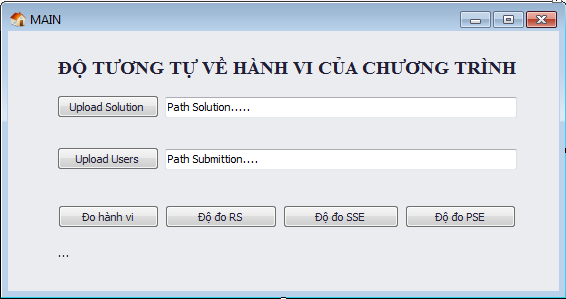
\includegraphics[width=\linewidth]{images/main.png}
  
\end{frame}

\begin{frame}
  \frametitle{Thực nghiệm}
%  \todo{mỗi cái cần giải thích dữ liệu liên quan}
%  -Thêm 1 slide giới thiệu 2 đoạn code, xem tương tự như thế nào, sau đó đến cái slide kết quả các phép đo.
%  - Thêm hai đoạn code 2 bên, giải thích hai đoạn code tính độ tương tự để có kết quả như hình bên dưới
  \begin{minipage}[t]{0.32\linewidth}
  	\centering
  	\lstinputlisting[basicstyle=\tiny]{CT_Thamchieu.cs}
  \end{minipage}%
  \hfill\vrule\hfill
  \begin{minipage}[t]{0.32\linewidth}
  	\centering
  	\lstinputlisting[basicstyle=\tiny]{Hocsinh1.cs}
  \end{minipage}%
  \hfill\vrule\hfill
  \begin{minipage}[t]{0.32\linewidth}
  	\centering
  	\lstinputlisting[basicstyle=\tiny]{Hocsinh2.cs}
  \end{minipage}%
	\pause
	\begin{itemize}
		\item Sub1 khác biệt hành vi: $ x = 2$ \pause
		\item Sub2 khác biệt hành vi: $ x = \{2, 3\}$
	\end{itemize}
\end{frame}

\begin{frame}
\frametitle{Kết quả phép đo RS}
\centering 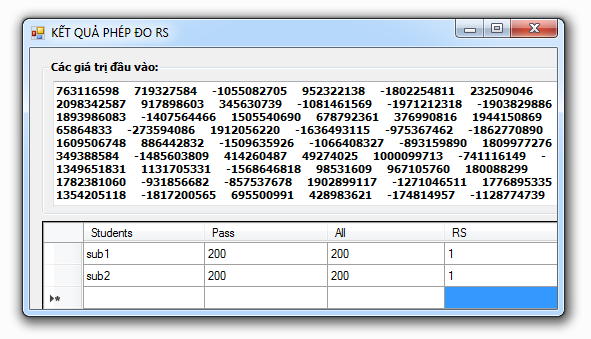
\includegraphics[width=0.8\linewidth]{images/kq_rs.png}
\begin{itemize}
	\item Lấy ngẫu nhiên 200 giá trị trên miền vào
	\item Độ tương tự hành vi bằng 1
\end{itemize}
\end{frame}

\begin{frame}
\frametitle{Kết quả phép đo SSE}
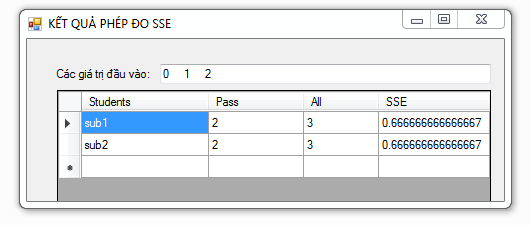
\includegraphics[width=0.8\linewidth]{images/kq_sse.png} 
\begin{itemize}
	\item $ DSE(P_r) = \{0, 1, 2\} $
	\item $ M_{SSE}= 0.66 $
\end{itemize}
\end{frame}

\begin{frame}
\frametitle{Kết quả phép đo PSE}
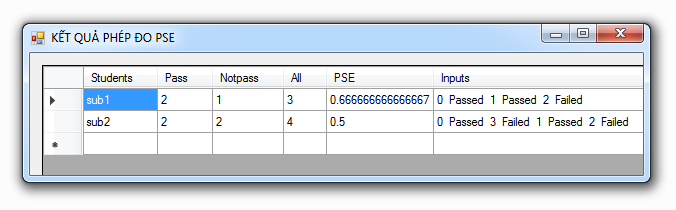
\includegraphics[width=1.0\linewidth]{images/kq_pse.png}
\begin{itemize}
	\item Hàm Sub1: $ DSE(P_{c}) = \{0, 1, 2\} $, $ M_{PSE}= 0.66 $
	\item Hàm Sub2: $ DSE(P_{c}) = \{0, 1, 2, 3\} $, $ M_{PSE}= 0.5 $
\end{itemize}
\end{frame}

\begin{frame}
  \frametitle{Kết luận}
%  \todo{Còn thiếu, đầu tiên phải nói những thứ mình làm}
	
  \begin{itemize}
  	\item Kết quả đạt được 
  	\begin{itemize}
  		\item Kiến thức cơ sở: testing, DSE
  		\item Các phép đo RS, SSE, PSE
  		\item Xây dựng cộng cụ hỗ trợ
  	\end{itemize} \pause
  	\item Hướng phát triển
  	\begin{itemize}
  		\item Cải tiến các phép đo để kết quả được chính xác hơn
  		\item Hỗ trợ một số ngôn ngữ Java, C++...
  	\end{itemize} \pause
  	\item Khả năng áp dụng
  	\begin{itemize}
  		\item Đánh giá tiến bộ trong lập trình
  		\item Xếp hạng tự động
%  		\item Gợi ý giải pháp lập trình
  	\end{itemize}
  \end{itemize}
\end{frame}


\part{}

\begin{frame}
  \frametitle{Tài liệu tham khảo}
% \todo{Còn cách nào đẹp hơn không????, chưa khớp với những nghiên cứu liên quan}
  \bibliographystyle{plain}
  {\footnotesize\bibliography{biblio}}
\end{frame}

\part{}
\begin{frame}
%  \todo{Sửa lại cho lịch sự hơn}
%  \todo{Sau khi hoàn thành hãy thêm hiệu ứng cho một số slides}
  \begin{center}
    \begin{Huge}
      \textcolor{BlueGreen}{\textbf{TRÂN TRỌNG \\ CẢM ƠN QUÝ THẦY CÔ!}}
    \end{Huge}
\end{center}

\end{frame}

% Tài liệu tham khảo

\end{document}



%%% Local Variables:
%%% mode: latex
%%% TeX-master: t
%%% End:
